% Propuesta de solución (documento final para la feria). Resume cap. 5-8.
\subsection{Descripción general de la solución}\label{sec:feria_solucion}

La solución es el sistema \textbf{ComedorUAGRM}, compuesto por un panel web para la gestión administrativa de la DUBSS, una aplicación móvil para los estudiantes y un módulo de Inteligencia Artificial que precalifica cada postulación. El flujo completo es: (a) la DUBSS publica una convocatoria; (b) el estudiante postula en línea y adjunta sus documentos en formato digital; (c) el módulo de IA calcula un puntaje de vulnerabilidad socioeconómica para el 100\% de las solicitudes; (d) la DUBSS audita únicamente a los finalistas mejor puntuados y adjudica las becas, generando el acta; (e) se controla la asistencia diaria de los becados y (f) las autoridades consultan indicadores de Business Intelligence.

El puntaje total (máximo 100) se obtiene sumando el puntaje de la IA (hasta 70) y el rendimiento académico verificado por el auditor (hasta 30). De este modo, los expedientes que se revisan físicamente dejan de depender del orden de llegada o del azar.

\subsection{Arquitectura y subsistemas}\label{sec:feria_arquitectura}

El sistema sigue una arquitectura cliente-servidor en capas, desplegada con Docker Compose: clientes web (React y TypeScript) y móvil (Flutter); una API REST en Java 21 y Spring Boot organizada en seis subsistemas; un módulo de preselección en Python con FastAPI, accesible solo desde la API; y una base de datos PostgreSQL con migraciones Flyway. Los archivos se almacenan en MinIO, y el tablero BI se alimenta de vistas materializadas de la misma base. La Figura~\ref{fig:feria_cu} muestra los casos de uso, la Figura~\ref{fig:feria_componentes} los componentes y la Tabla~\ref{tab:feria_subsistemas} los subsistemas.

\begin{table}[H]
\caption{Subsistemas de la solución y casos de uso que los conforman}
\label{tab:feria_subsistemas}
\centering
\footnotesize\linespread{1}\selectfont
\renewcommand{\arraystretch}{1.3}
\begin{tabular}{>{\raggedright\arraybackslash}p{5.5cm}>{\raggedright\arraybackslash}p{9.5cm}}
\toprule
\textbf{Subsistema} & \textbf{Casos de uso} \\
\midrule
Cuentas y Acceso & CU01, CU14, CU15 \\
Convocatoria y Postulación & CU13, CU02, CU16, CU17, CU18, CU04 \\
Preselección con IA & CU03, CU26 \\
Auditoría y Adjudicación & CU05, CU06, CU07, CU08, CU19, CU20, CU21, CU22 \\
Becados y Asistencia & CU23, CU09, CU10, CU11, CU24 \\
Reportes y Trazabilidad & CU12, CU25 \\
\bottomrule
\end{tabular}

\smallskip
\noindent\raggedright\textit{Nota.} Elaboración propia.
\end{table}

\begin{figure}[H]
\caption{Diagrama general de casos de uso del sistema}
\label{fig:feria_cu}
\centering
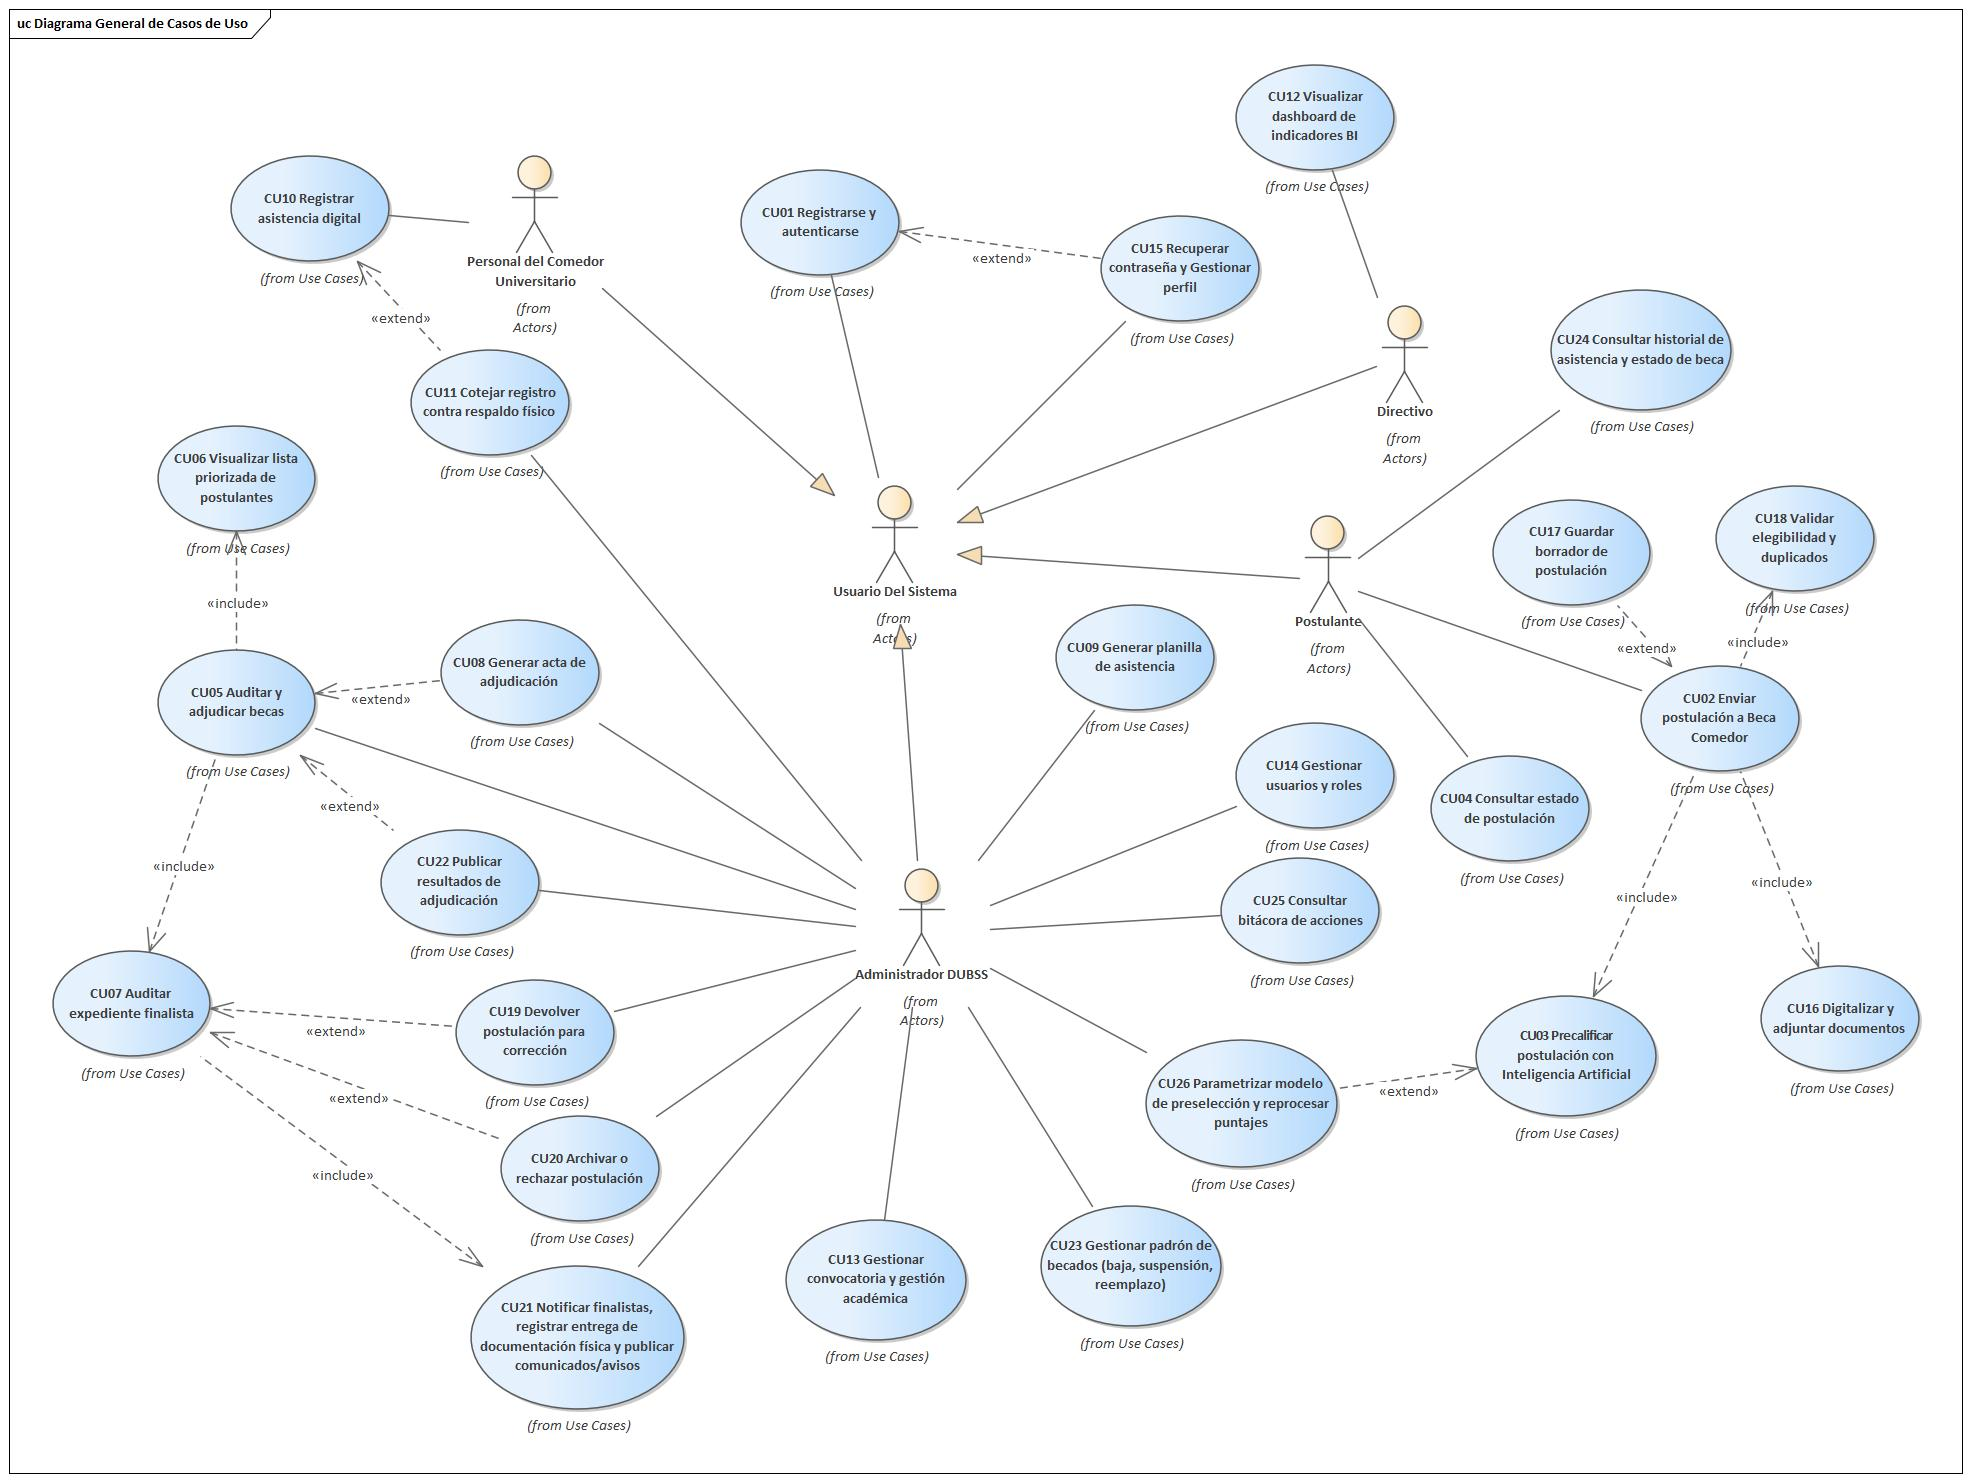
\includegraphics[width=\textwidth,height=0.45\textheight,keepaspectratio]{images/019_Diagrama_General_CU.jpg}

\smallskip
\noindent\raggedright\textit{Nota.} Elaboración propia.
\end{figure}

\begin{figure}[H]
\caption{Diagrama de componentes del sistema completo}
\label{fig:feria_componentes}
\centering
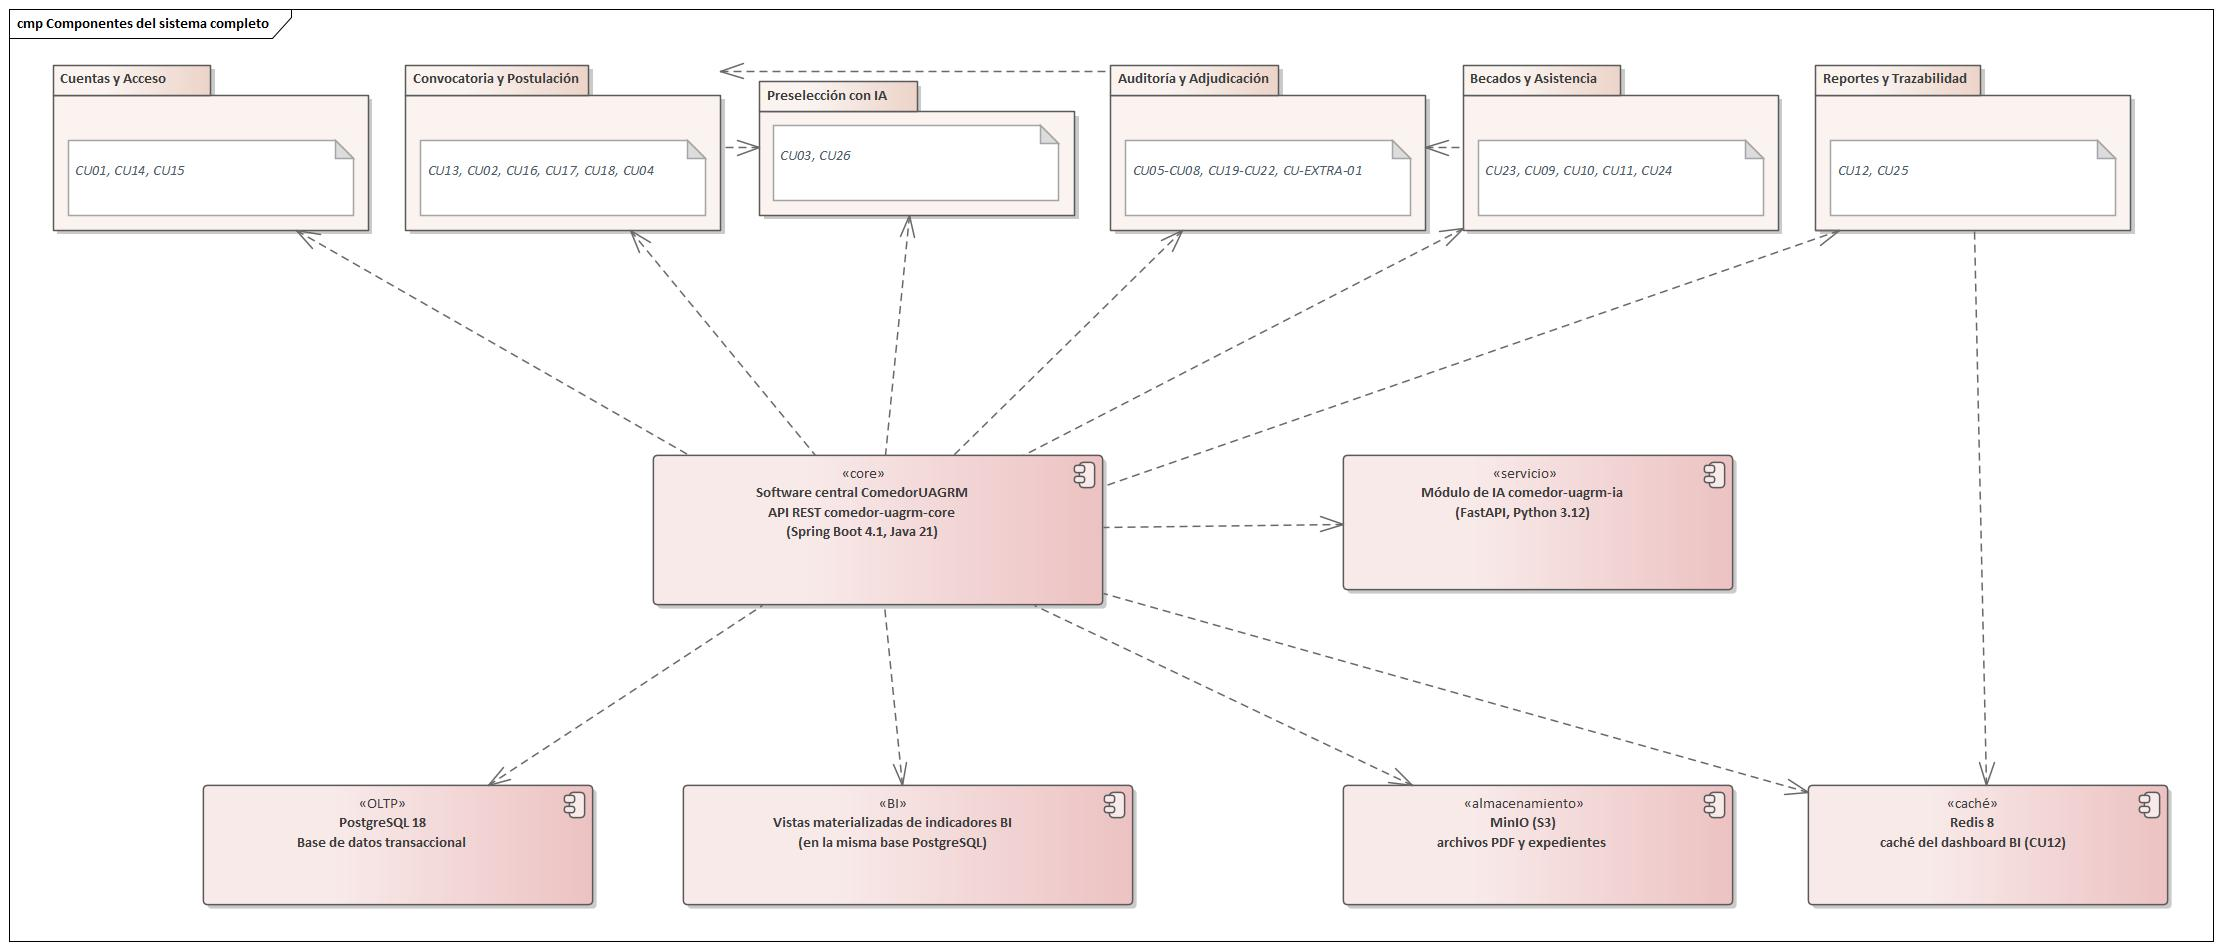
\includegraphics[width=\textwidth,height=0.45\textheight,keepaspectratio]{images/147_Componentes_Sistema_Completo.jpg}

\smallskip
\noindent\raggedright\textit{Nota.} Elaboración propia.
\end{figure}

\subsection{Funcionalidades principales}\label{sec:feria_funcionalidades}

\begin{itemize}
    \item \textbf{Postulación en línea:} registro, formulario socioeconómico, carga de documentos, guardado de borrador y consulta del estado de la solicitud (CU01, CU02, CU16, CU17, CU04).
    \item \textbf{Preselección con IA:} validación de elegibilidad y duplicados, cálculo del puntaje de vulnerabilidad y parametrización del modelo (CU18, CU03, CU26).
    \item \textbf{Auditoría y adjudicación:} lista priorizada de finalistas, auditoría del expediente, devolución o archivo, acta de adjudicación y publicación de resultados (CU05--CU08, CU19--CU22).
    \item \textbf{Control de asistencia:} padrón de becados, asistencia digital, planillas imprimibles y cotejo con el respaldo físico (CU23, CU10, CU09, CU11).
    \item \textbf{Business Intelligence y trazabilidad:} dashboard de indicadores y bitácora de acciones (CU12, CU25).
\end{itemize}

La Figura~\ref{fig:feria_mock} muestra las interfaces de la precalificación con IA y del dashboard BI.

\begin{figure}[H]
\caption{Interfaces del sistema: precalificación con IA (CU03) y dashboard de indicadores BI (CU12)}
\label{fig:feria_mock}
\centering
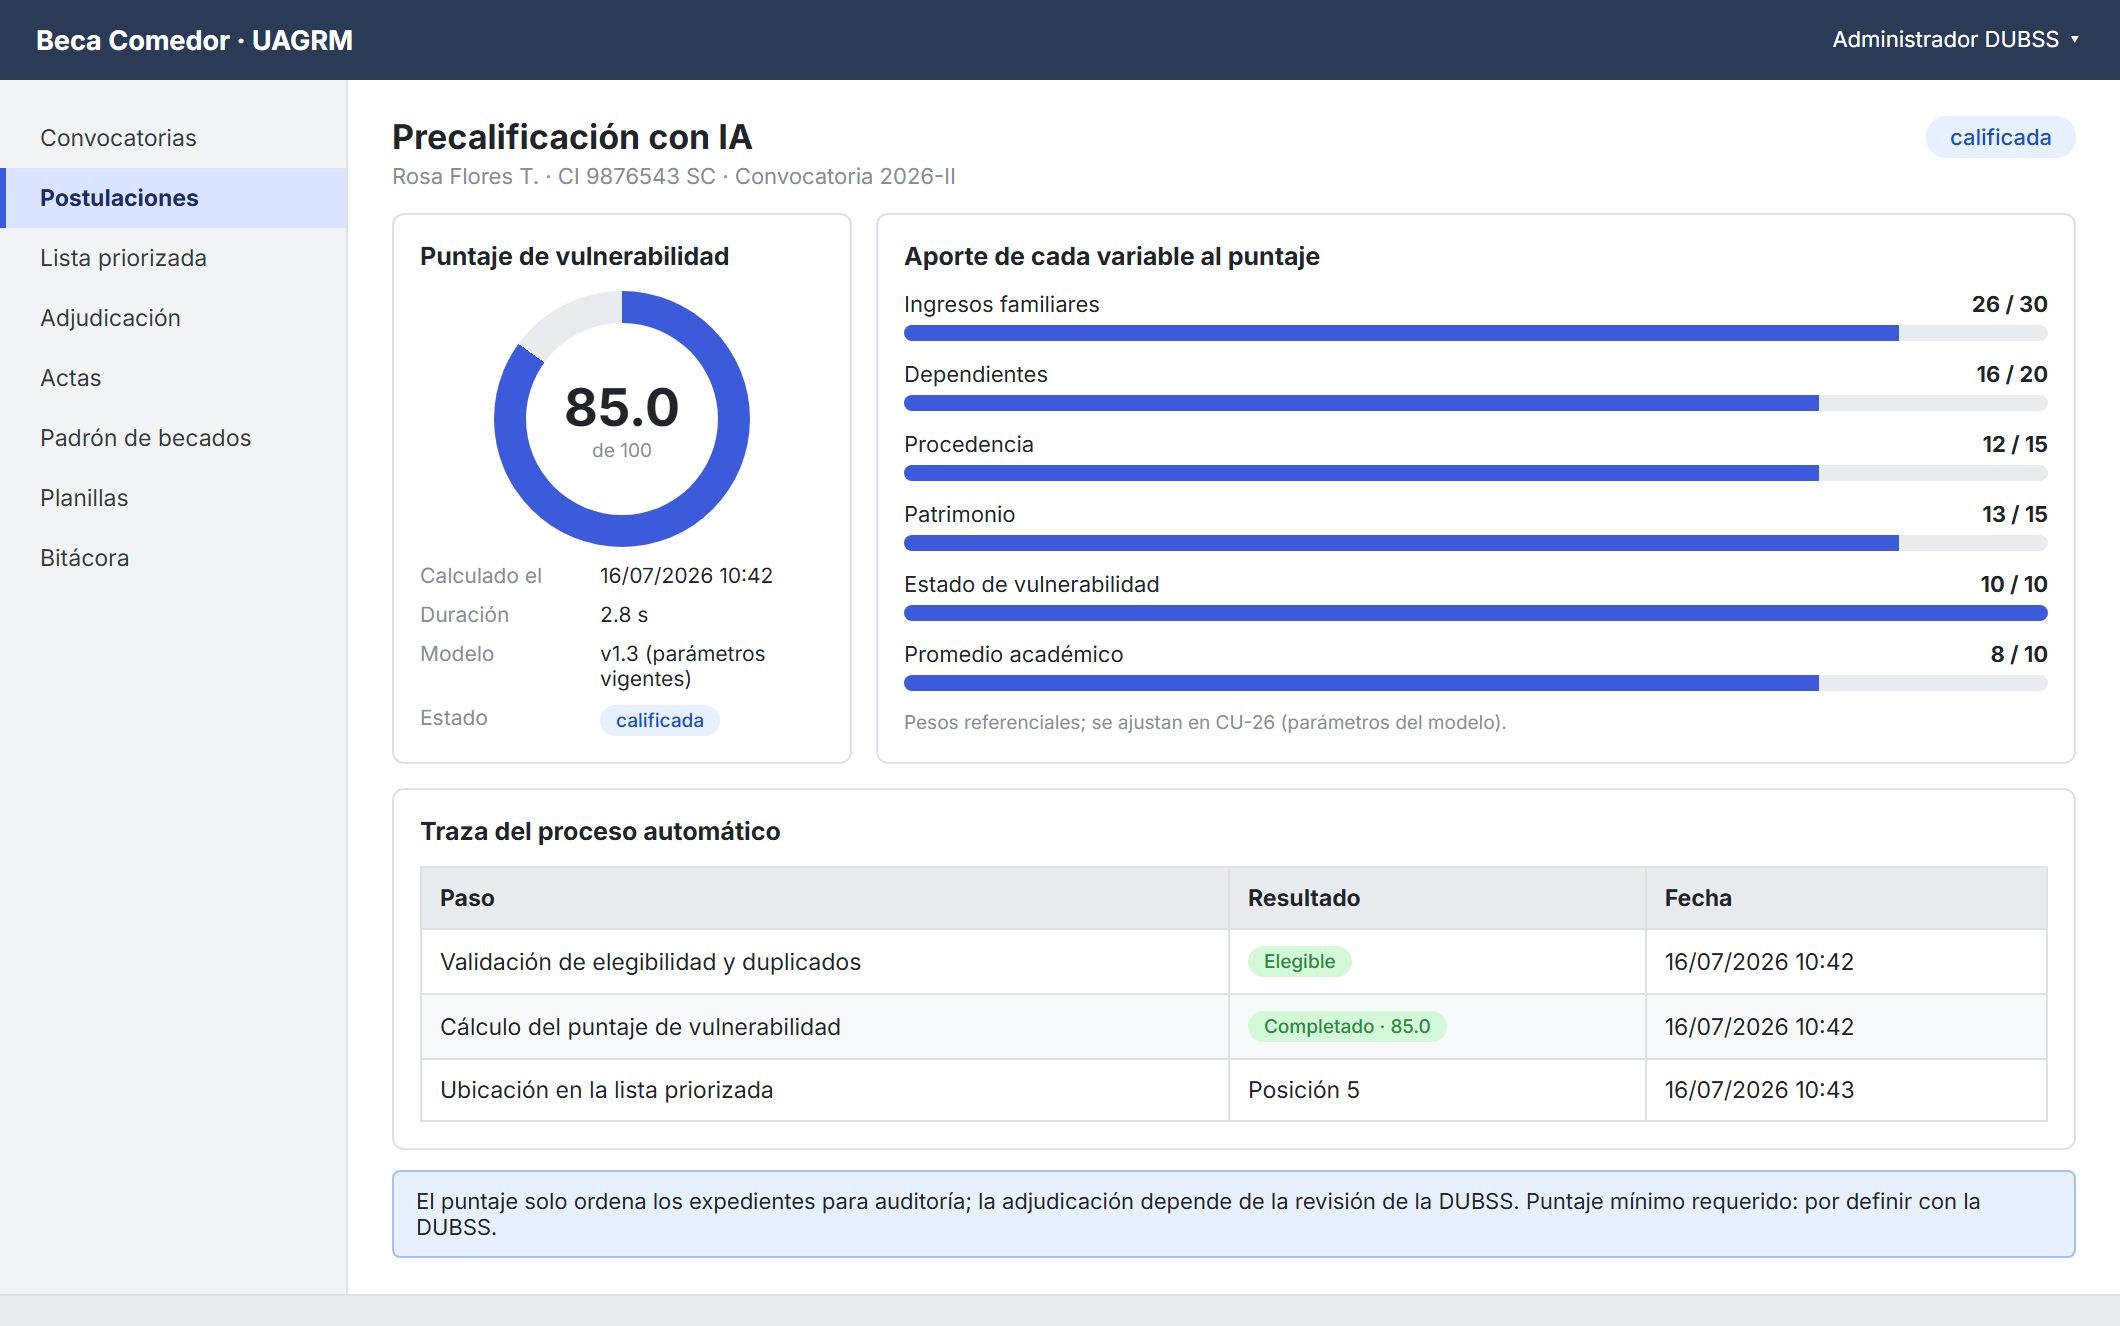
\includegraphics[width=0.48\textwidth]{images/136_Mockup_CU03_Precalificar_IA.png}\hfill
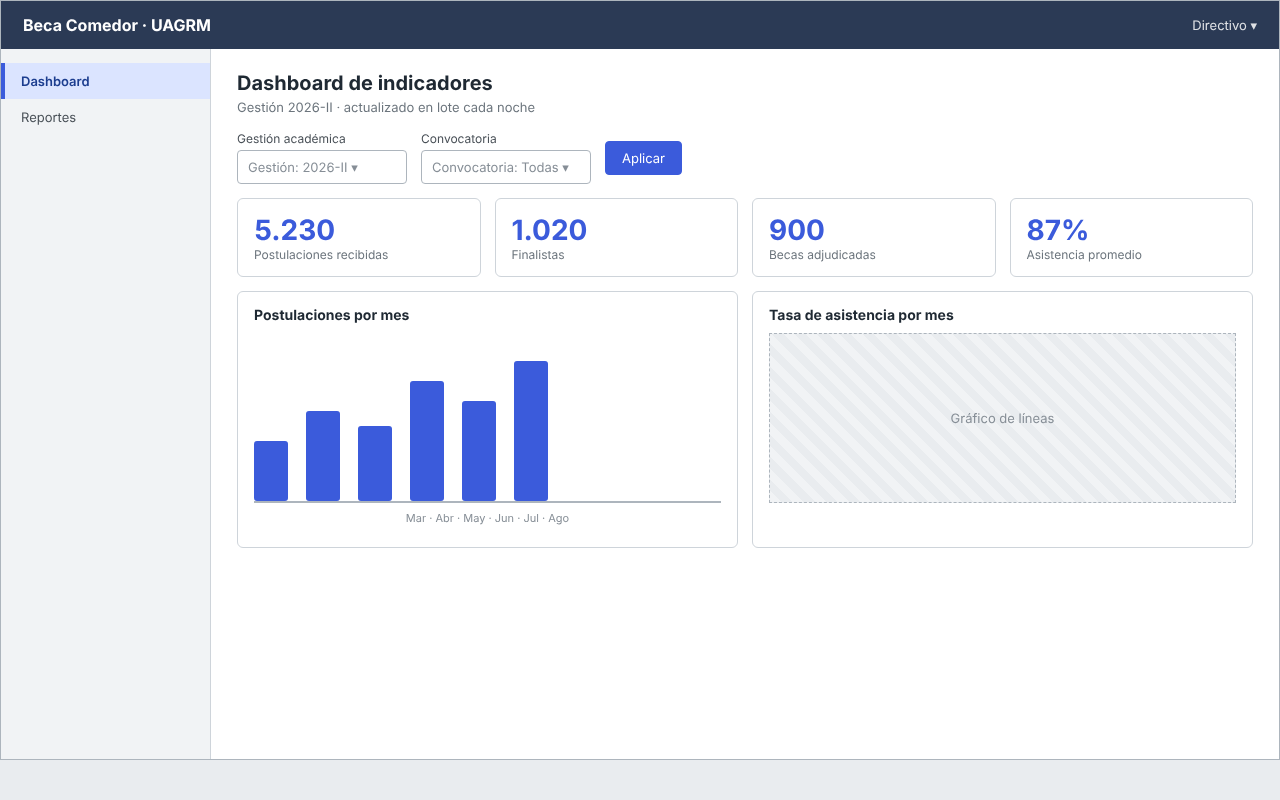
\includegraphics[width=0.48\textwidth]{images/112_Mockup_CU12_Dashboard_BI.png}

\smallskip
\noindent\raggedright\textit{Nota.} Elaboración propia.
\end{figure}
